\chapter{ Results }

During this chapter the questions initially stated are going to be study in detail, 
looking forward to answer them. Though there are several questions, the central one
consists in finding if there is any difference in BAO properties when the scale of the tracer
halo population is changed. A possible way to account for this, it is to study the 
clustering at BAO scales for such halo populations. That is precisely what is proposed
in this work. 
One statistical tool that will be used to study clustering were already explained in chapter \ref{chap3},
the correlation function will provide our main results. 

\

Now, using this tool, the simulation Multidark Planck (MDPL) will be studied. 
It belongs to the MultiDark database in which Planck parameters were used
(table \ref{plancktable}). The characteristics of MDPL
simulation are a box length of $L=1$Gpc/h, a number of particles equal to 
$3840^3$ and a mass resolution of $1.51e9 M_{\odot}/h$.
Furthermore, the MDPL simulation has available a halo catalogue constructed with Friend of 
Friends algorithm and a linking length of 0.2 \footnote{ Data taken from \url{https://www.cosmosim.org/cms/simulations/MDPL/}}. 
From this halo catalog are constructed several populations using the mass of the halos to
classify them. This is more clear from the table \ref{pophalos} where each mass range for 
the 4 different populations constructed are shown. They are going to be called the 
thick bins. 

But, the populations have a range mass that is arbitrary, so
the results obtained can have some sort of bias. To avoid this, 
it will be study in further detail the effect that 
the size of the mass bins have in the results, i.e., the mass
range considered. The bins size could be ``masking'' information
contained for smaller mass ranges. 	

Hence, there are other subsamples created from every thick bin.
Four populations are constructed for the population $1$,  
each of them has the same number of halos. %as shown in figure \textit{pendiente}. 
They are labelled as $q_i$ with $i=1,\dots,4$, $q_1$ is the extreme 
nearer to population 3 and $q_4$ is the extreme nearer to population 1. 
Likewise, for the population $2$ other four populations are constructed where
the same labelling is used. They will be called quarter populations. 
There was another reason to construct such populations, the correlation function
found for the population 2 has an irregular shape around values of BAO peak. This
will later discussed in a next section. 
Aditionally, other bins called the thin bins are created. The mean mass for each 
bin are $10^{12.5}, 10^{12.9}, 10^{13.3}, 10^{13.7}, 10^{14.1}, 10^{14.5}$ and $10^{15}$. 

Concluding, all of these subdivisions are created to study the effect of the scale of the populations 
on the BAO signal. This is found to be related with the nonlinear gravitational effects, i.e.
for smaller mass halos there is a coupling among different density modes. 

This lead us to other experiment, to revise if there is a difference in the BAO properties
found for the same cosmological box but for $z=1$, where nonlinear gravitational effects
should be less prominent. In the table \ref{z1}, it is going to be shown populations used 
for $z=1$. The same procedure that will be exposed for the populations with $z=0$ is followed
for $z=1$, but we are going to concentrate in the first redshift where a deeper study 
was performed. 

\begin{table}
\begin{center}
  \begin{tabular}{ | c | c | c | }
    \hline \hline
    MDPL population & Mass range $M_{\odot}$& Number of halos \\ \hline \hline
    4 & $ M \geqslant 1e14$ & 32436 \\ \hline
    3 & $ 1e13 \leq M < 1e14 $ & 443356\\ \hline
    2 & $ 1e12 \leq M < 1e13$ & 3687677\\ \hline
    1 & $ 1e11 \leq M < 1e12$ & 32868688 \\ \hline
  \end{tabular}  
   \caption{ Populations constructed from the mass range that appears in column two (z=0). }
\label{pophalos}
\end{center}
\end{table}


\begin{table}
\begin{center}
  \begin{tabular}{ | c | c | c | }
    \hline \hline
    MDPL population & Mean Mass $M_{\odot}$& Number of halos \\ \hline \hline    
    9 & $ 1e13.5$ & 8462\\ \hline
    8 & $ 1e13$ & 66473 \\ \hline
    7 & $ 1e12.5$ & 326163 \\ \hline
    6 & $ 1e12$ & 1258759 \\ \hline
    5 & $ 1e11.5$ & 4333890 \\ \hline
  \end{tabular}  
   \caption{ Populations constructed for $z=1$. }
\label{z1}
\end{center}
\end{table}



\section{ Correlation functions for MDPL populations}


\begin{figure}[htbp]
   %\begin{center}
   $
    \begin{array}{ll}
    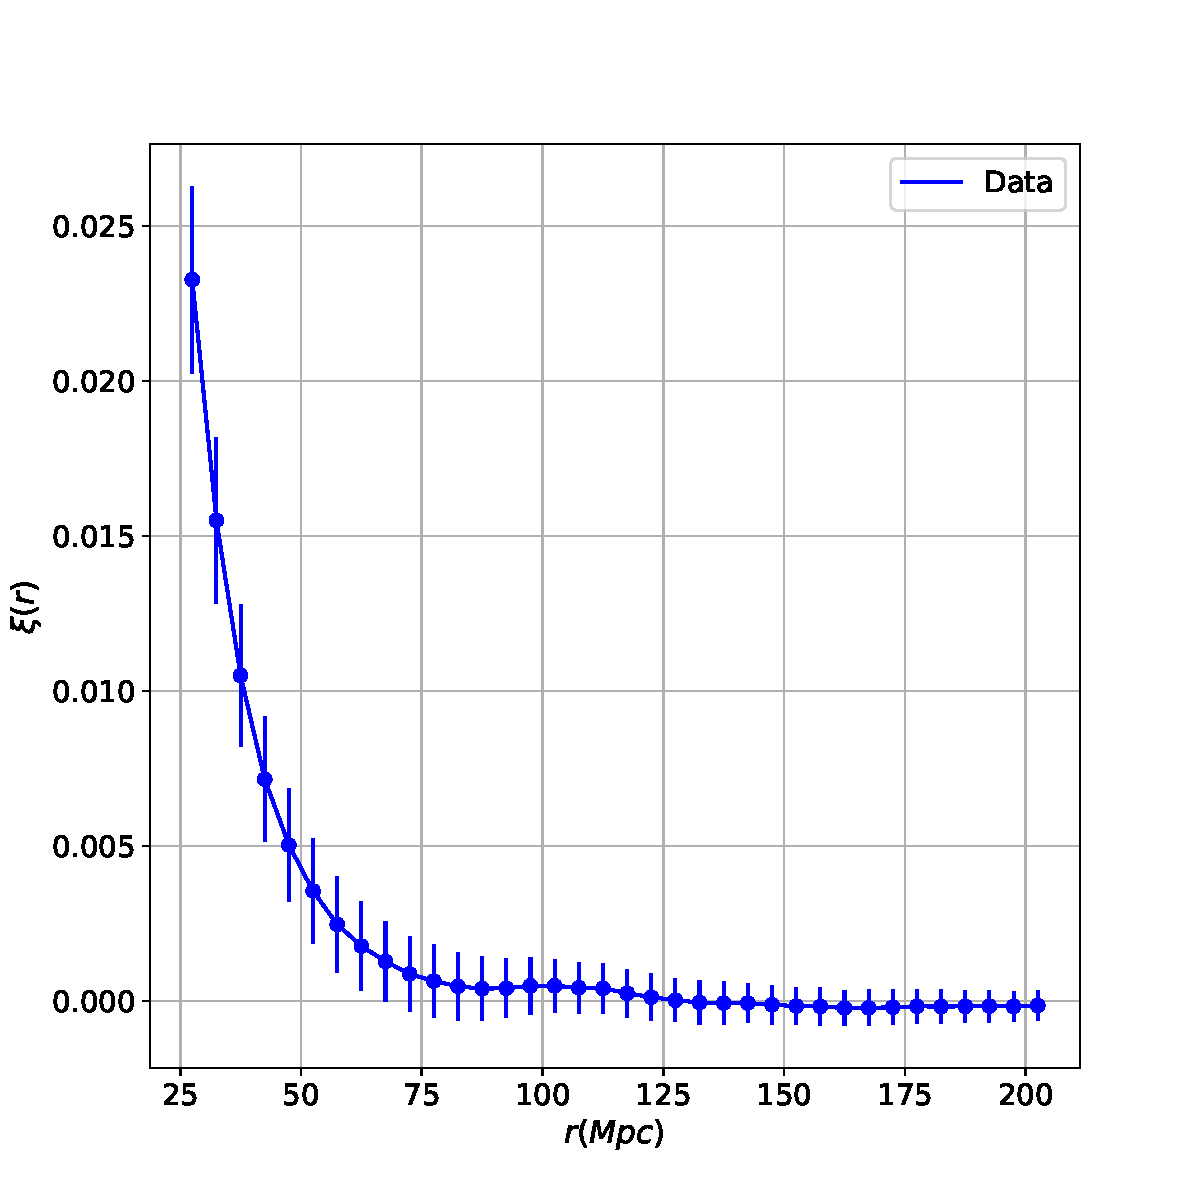
\includegraphics[width=85mm]{Images/chapter4/CF_all_1e11.pdf}&
    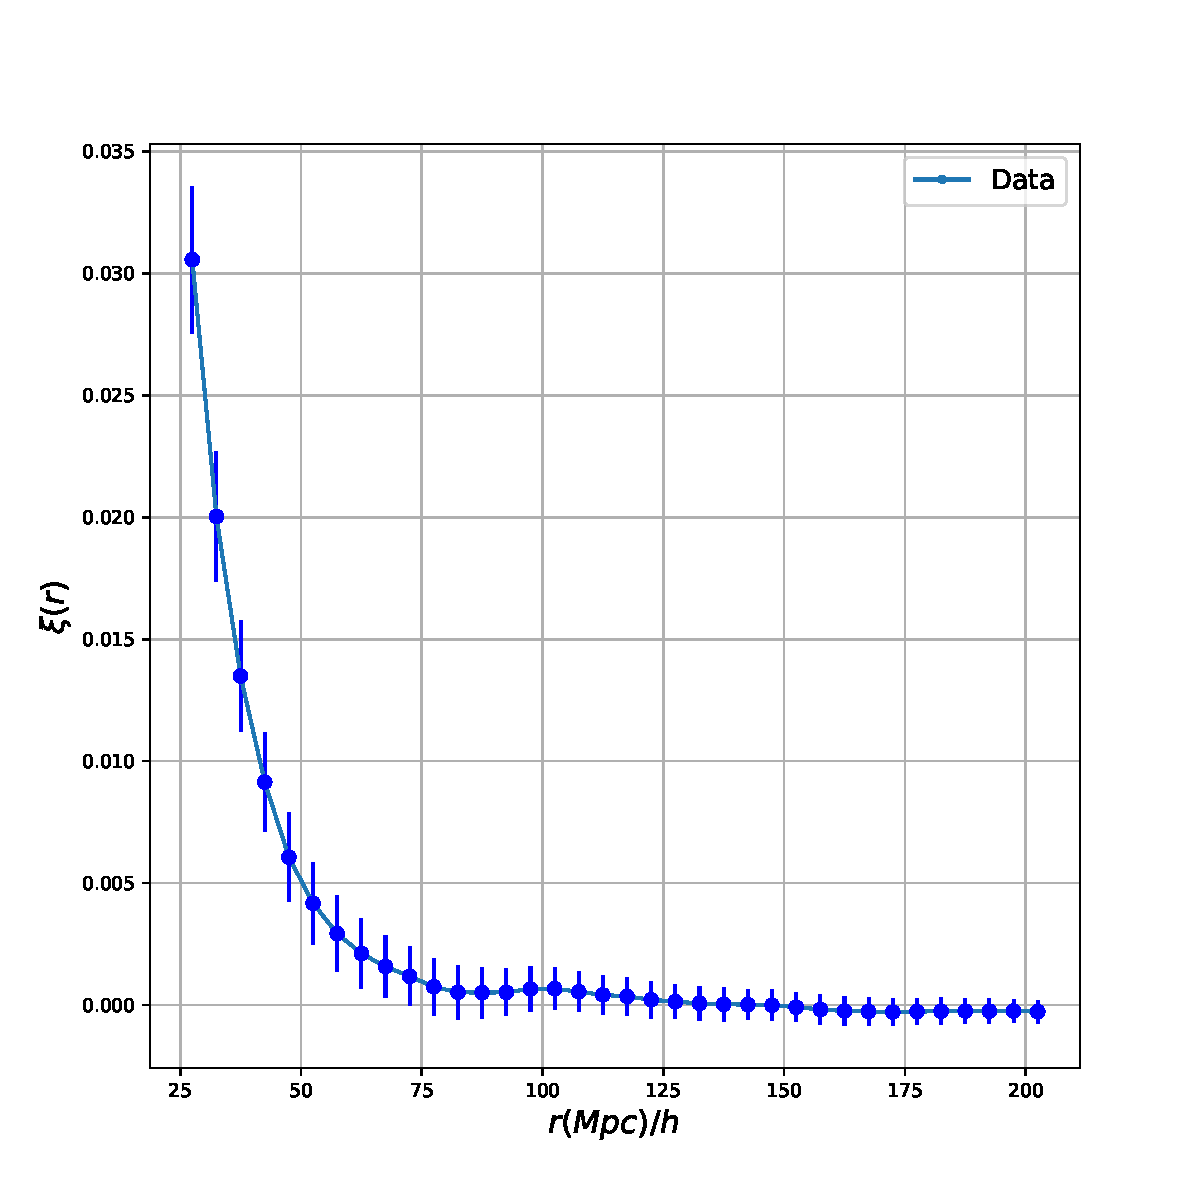
\includegraphics[width=85mm]{Images/chapter4/CF_all_1e12.pdf}\\
    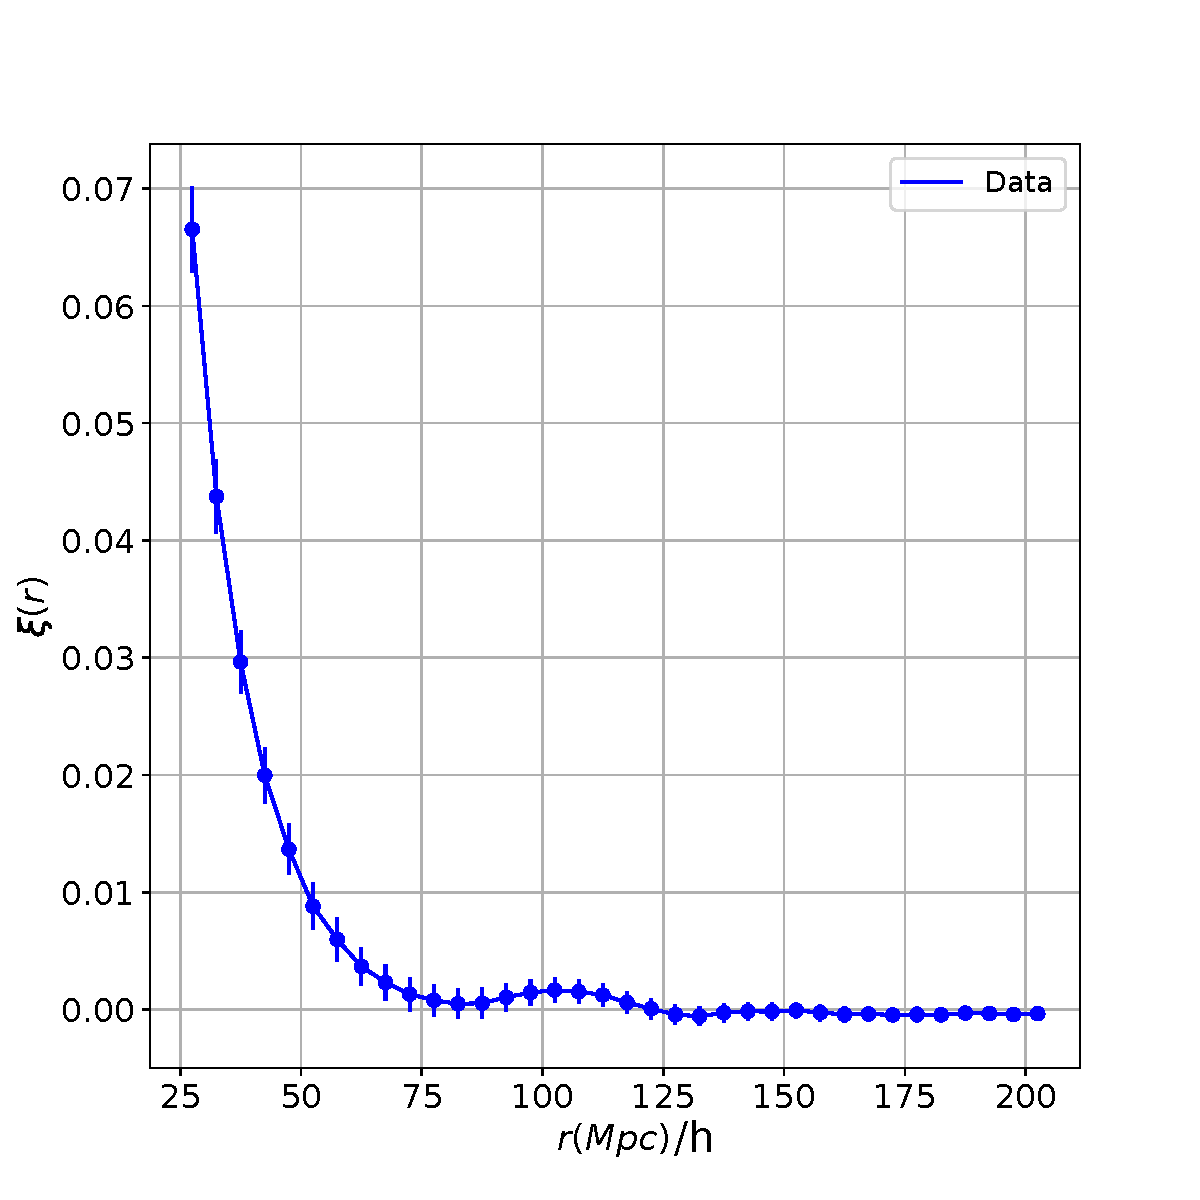
\includegraphics[width=85mm]{Images/chapter4/CF_all_1e13.pdf}&
    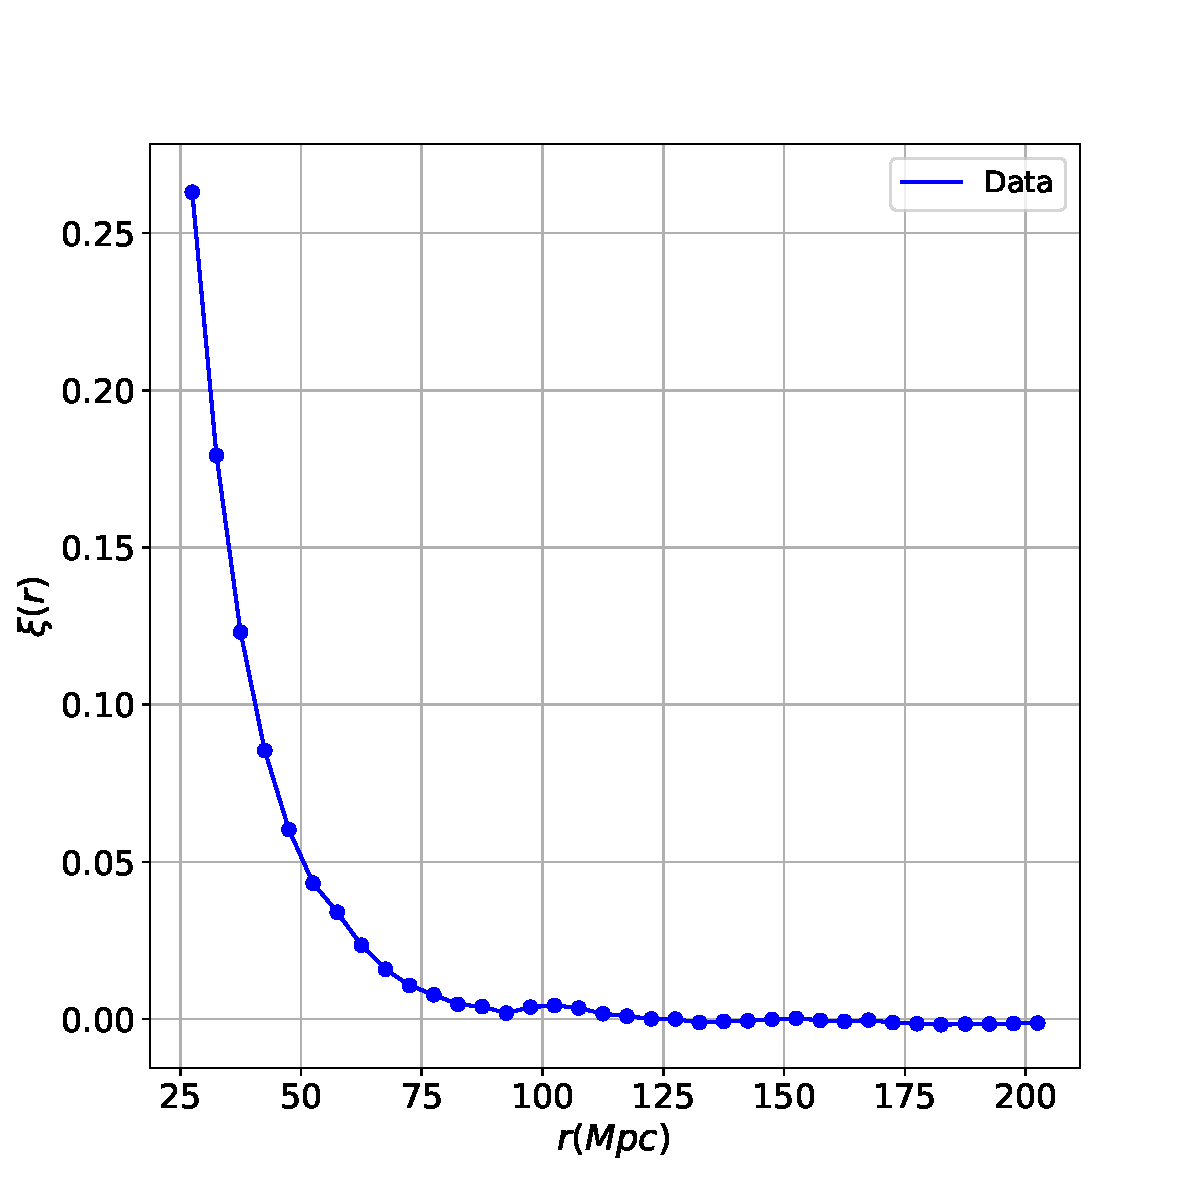
\includegraphics[width=85mm]{Images/chapter4/CF_all_1e14.pdf}
    \end{array}$
  %\end{center}
   \caption{The correlation functions for populations $1$ with $N_{random} =10$, $2$ with $N_{random} =10$, $3$ with with $N_{random} =10$ and $4$ with with $N_{random} =40$ are displayed from the upper left to the lower right. For each population 3 runs with 12 bins were performed. }
   \label{CFall}
\end{figure}


To calculate the correlation function was implemented a parallel C code 
that uses mpi.
There are several important quantities in order to run the code
and obtain the correlation function for a specific population, 
the random sample factor $N_r$, the minimum radial value $R_{min}$, 
the maximum radial value $R_{max}$, the radial number of bins $N_{bins}$,
and the number of particles of the population $N_{part}$.
The random sample factor accounts for the size of the random-random 
catalogue, the total population for the RR catalogue is 
$N_r N_{part}$.
The quanties $R_{min}$ and $R_{max}$ define a range where correlation
function is found. With this range and the radial number of bins 
a distance is estimated, points where the correlation function is
computed.

Next, in the figures \ref{pophalos}, the correlation function for every population 
is shown. The random factor used is not the same for each case, 
it diminish with the bigger populations since it would be too expensive
computationally to use a big enough value for all of them. For each population 
3 different runs were performed with the same $N_r$ and $N_b = 12$. The first one used 
$R_{min}=20$ and $R_{max}=200$, the second one $R_{min}=25$ and $R_{max}=205$
and the last one $R_{min}=30$ and $R_{max}=210$. In this way the noise 
in the final correlation function plotted per population is reduced. 
This is, if only one run from $R_{min}=20$ to $R_{max}=210$ with bins width of $5$
Mpc would have been performed, less data would have been used to calculate the correlation function 
per bin compared with the 3 runs performed, making more robust the results in the last scenario. 

In the different figures the correlation function obtained has a similar 
shape and there is a bump around $\sim 105$ Mpc that corresponds
to the BAO peak. 
But there is a difference in the amplitude and the particular population. 
The more massive halo populations have a larger amplitude
compared with the lower ones. This is more clear from the maximum value obtained in
each case. 

Further, an error bar was found for each point where the correlation function 
was found. For this, 10 realizations with the same characteristics for each
population were calculated. The standard deviation found using the realizations
are the values used for the error bars. 
In the figures there are a decrease in the error bars for each population as they 
become more massive. Hence, the correlation function for the realizations are more alike 
for the smaller populations. 


\subsection{ Random Sampling and Number of particles}


Since the random sampling factor is intended to reduce the shot 
noise, it is important to study its impact on the calculation
of the correlation function (CF). A first exercise in this direction
is displayed in the figure \ref{nrandom} for the population 4, 
the correlation function was calculated for 3 different random sampling factors. 
There is something important to highlight, there were performed
ten realizations per $N_{r}$ and the CFs shown are the mean of these
realizations. From the figure what can be seen is that there is no 
significant change in the CF obtanied due to the random sampling number, 
not at least for radial values smaller than $150$ Mpc. 
For bigger values, the CF with a smaller random sampling factor 
behavior becomes a little bit noisier but this scales are not of our interest.

If the same exercise is repeated with specific realizations instead of the
mean CFs, more fluctuatios are introduced producing a more notorious difference
for scales smaller than $150$ Mpc. 

%**********************************************************************************************************************
\begin{figure}[htbp]
       \centering
               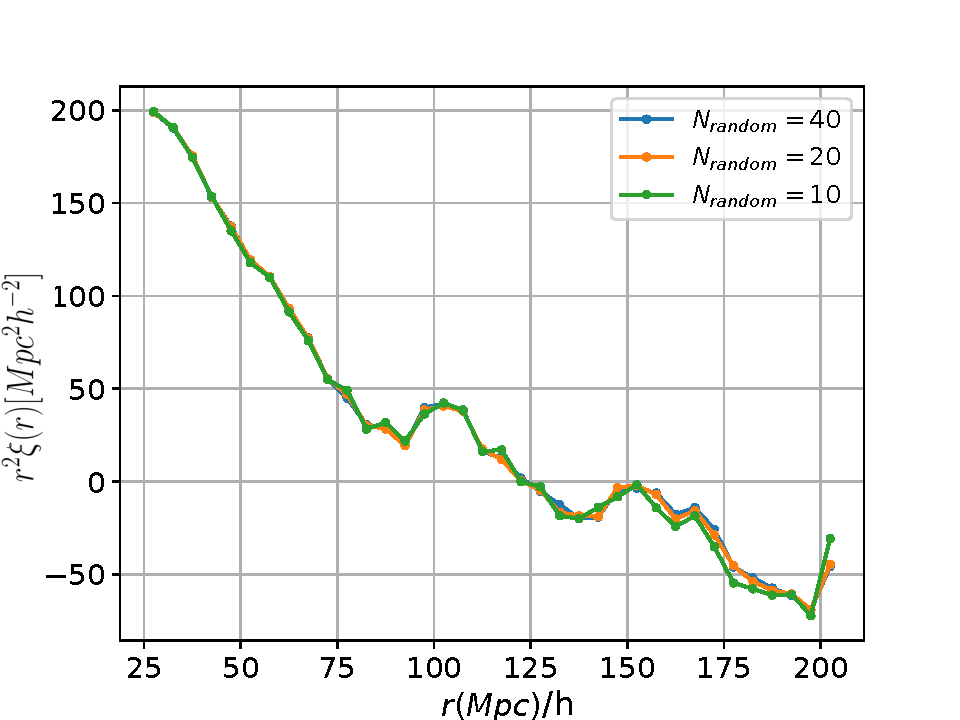
\includegraphics[width=0.7\textwidth]{Images/chapter4/CF_1e14_Nrandom.pdf}
       \caption{\small Correlation function for population 4 with different random factor
       numbers.}
       \label{nrandom}
 \end{figure}
%**********************************************************************************************************************


Other exercise performed to find the effect of the $N_r$ on the CF is shown
in the figure \ref{CFscat}. In this case, for a thick population, $10^{14.5}$
several realizations with the same characteristics were performed except
by the $N_r$ used. The two values for $N_r$ are 50 and 100 with equal number
of realizations per calculation. The plotted line in each CF corresponds to the 
mean of the realizations. The x range was reduced to see in more detail the
bump of the BAO. The dispertion of the CFs values for the two $N_r$ values
is very similar. Hence, there is no change in the CF estimation because of 
$N_r$ value.
Though the left figure appears with more points per bin, this is caused
because of the difference in the number of realizations done. 

\begin{figure}[htbp]
   %\begin{center}
   $
    \begin{array}{ll}
    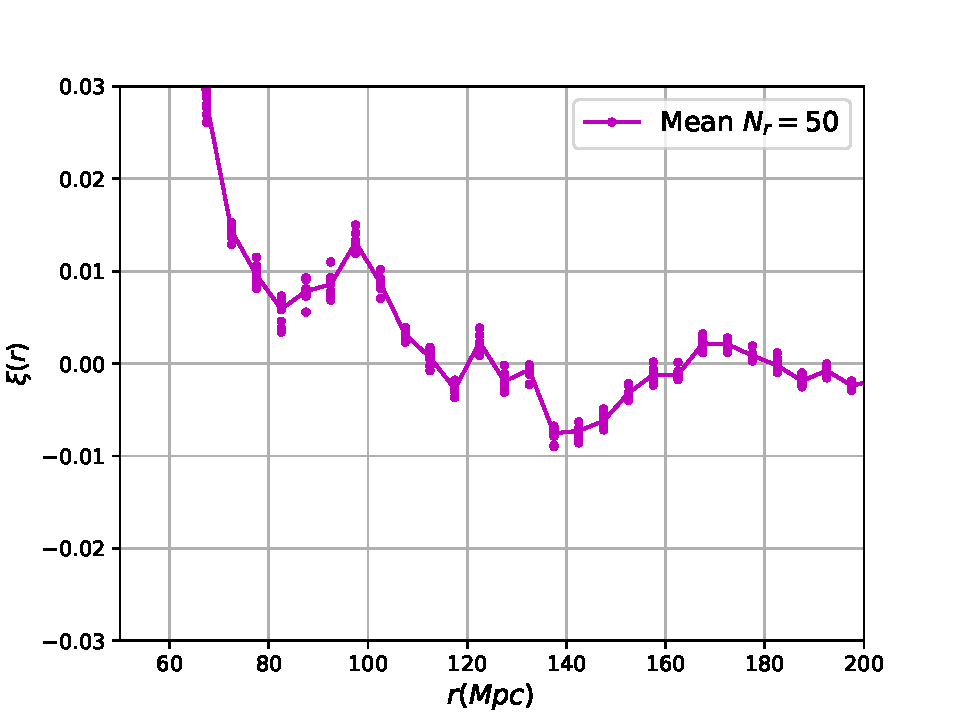
\includegraphics[width=80mm]{Images/chapter4/scatter_mean_1e145_50.pdf}&
    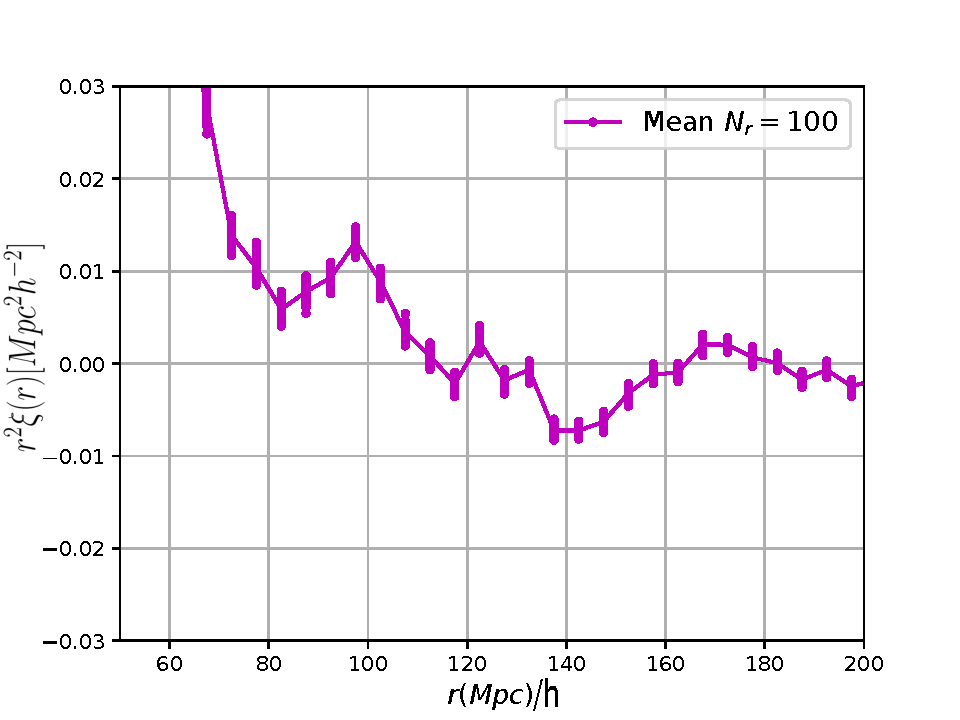
\includegraphics[width=80mm]{Images/chapter4/scatter_mean_1e145_100.pdf}
    \end{array}$
  %\end{center}
   \caption{Correlation function for population $14.5$ with two $N_r$ values.
   The left panel displays 50 different CFs and the right one 100 different CFs.}
   \label{CFscat}
\end{figure}


There was another factor that has to be considered, the number of particles taken for the 
correlation function calculation. Since there is a large number of particles for the 
population 1 and 2, there is not enough computational resources to run the program, hence
it is necessary to use a subsample representative of all of population. Now, the idea
is to study the effect it has on the estimation of the correlation function. 
In the figure \ref{NofP} is shown for the population 1 the correlation function obtained
for two different subsamples, one is around $7.6\%$ of the total population
and the other one is around $15.2\%$ percentage of the total population. Both
correlation functions coincide for ranges lower to $80$ Mpc, in the region where BAO.


%**********************************************************************************************************************
\begin{figure}[htbp]
       \centering
               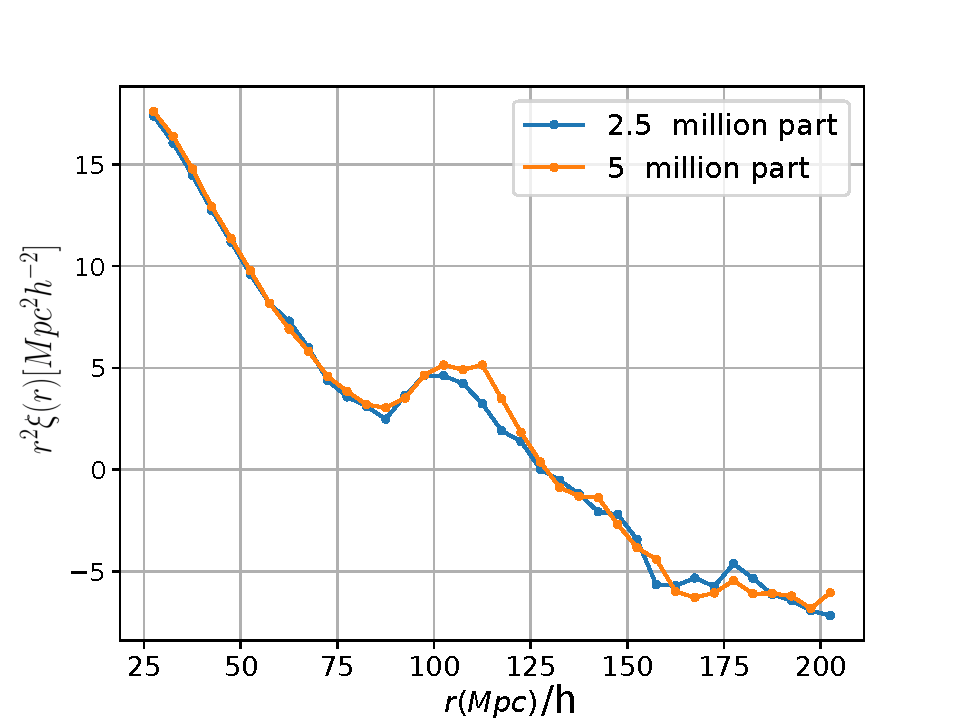
\includegraphics[width=0.7\textwidth]{Images/chapter4/CF_1e11_NofP.pdf}
       \caption{\small Correlation function for two different subsamples of population 
       population 1 .}
       \label{NofP}
 \end{figure}
%**********************************************************************************************************************



\section{ Correlation function fit }

A first step torward obtaining the BAO signal and its properties from the CF,
it is to make a fit precisely of the CF. In the figure \ref{CFall} the CF 
for different populations are shown, the label used for them is \textit{data}. 
As it can be seen the $y$ axis corresponds to $r^2\xi(r)$ since it allows to visualize better the BAO bump.

The CF function fits that we are finding do not try to reproduce 
the bumps observed in the correlation function. Because of this, not all 
the points obtained for a CF estimation were used to make the fit, only
those ones that do not fall in the bumps. 

The fit of the points were adjusted to the function 

\begin{equation}
f(r) = r^2\xi(r) = \frac{r^\lambda}{a_0}
\label{CF_r2}
\end{equation}

\begin{figure}[htbp]
   %\begin{center}
   $
    \begin{array}{ll}
    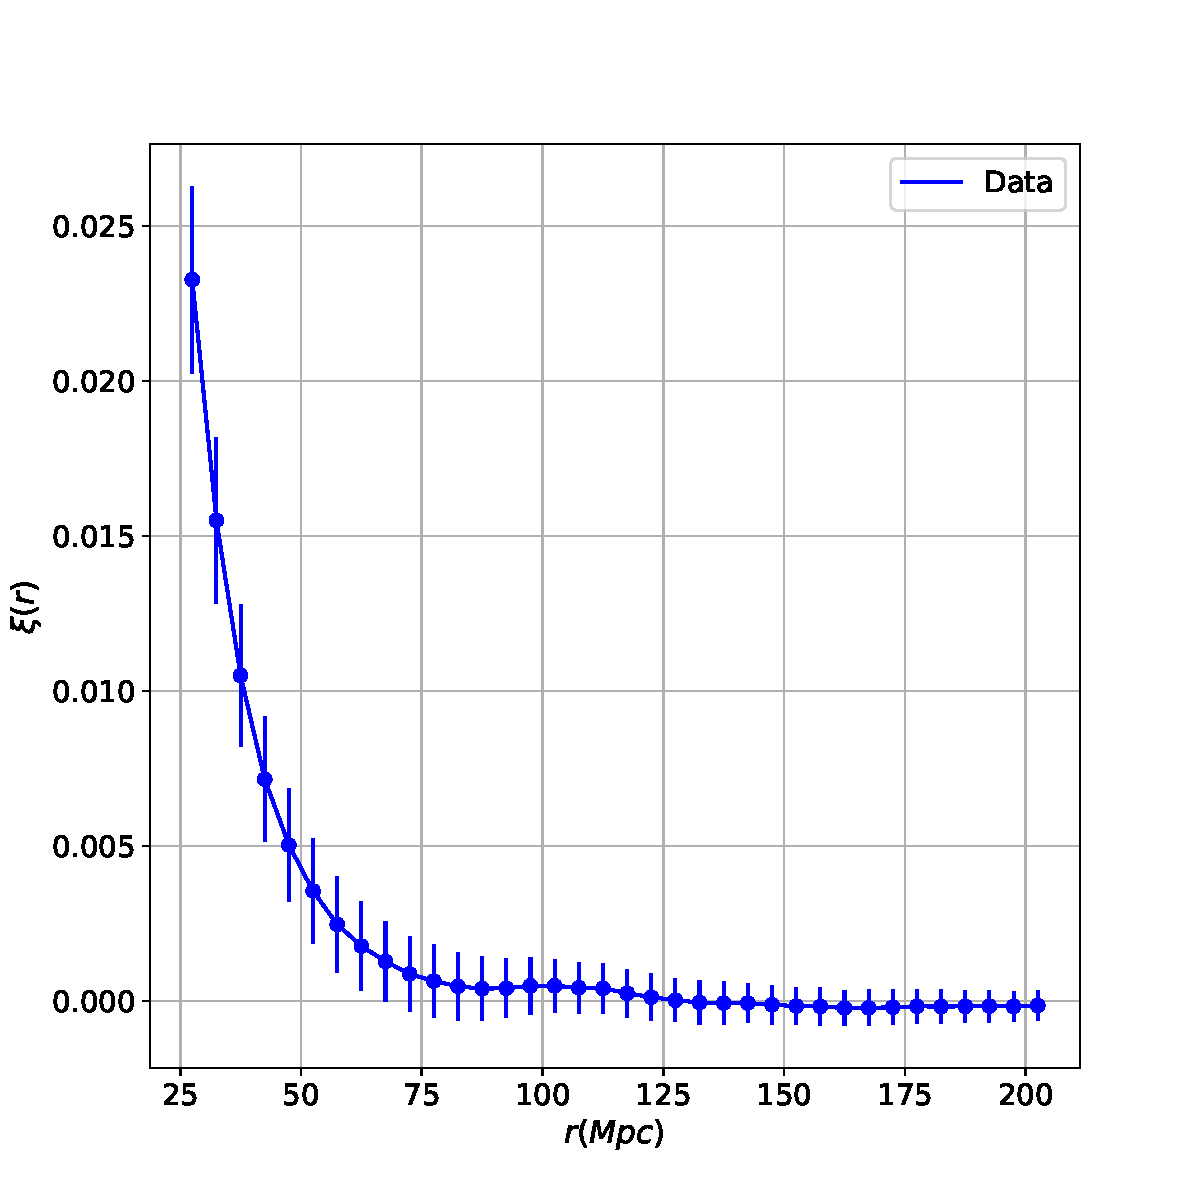
\includegraphics[width=85mm]{Images/chapter4/CF_all_1e11.pdf}&
    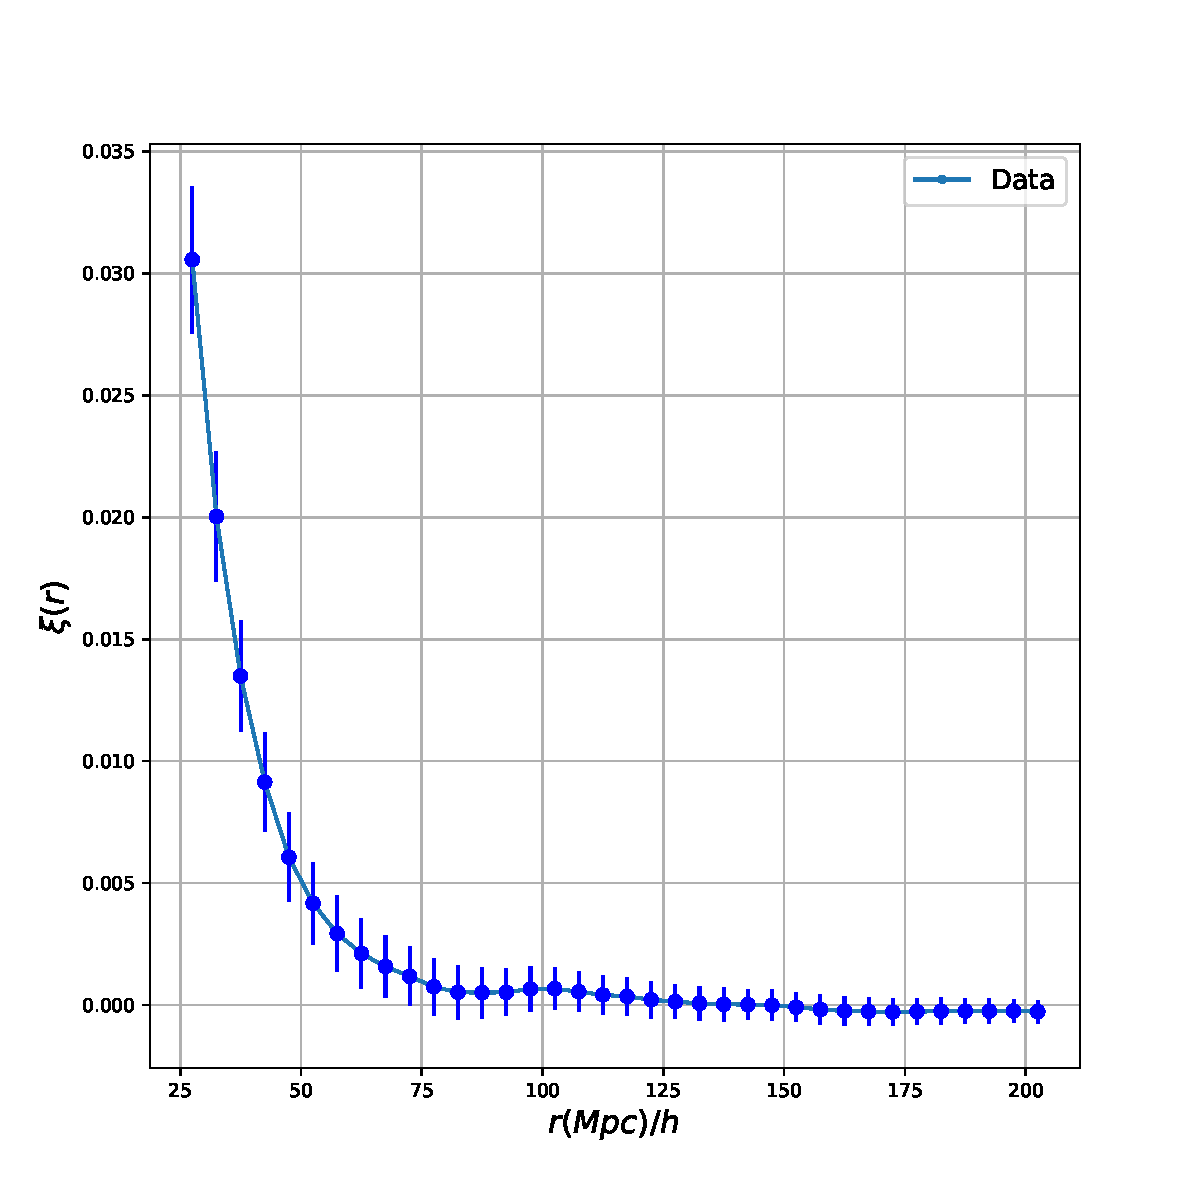
\includegraphics[width=85mm]{Images/chapter4/CF_all_1e12.pdf}\\
    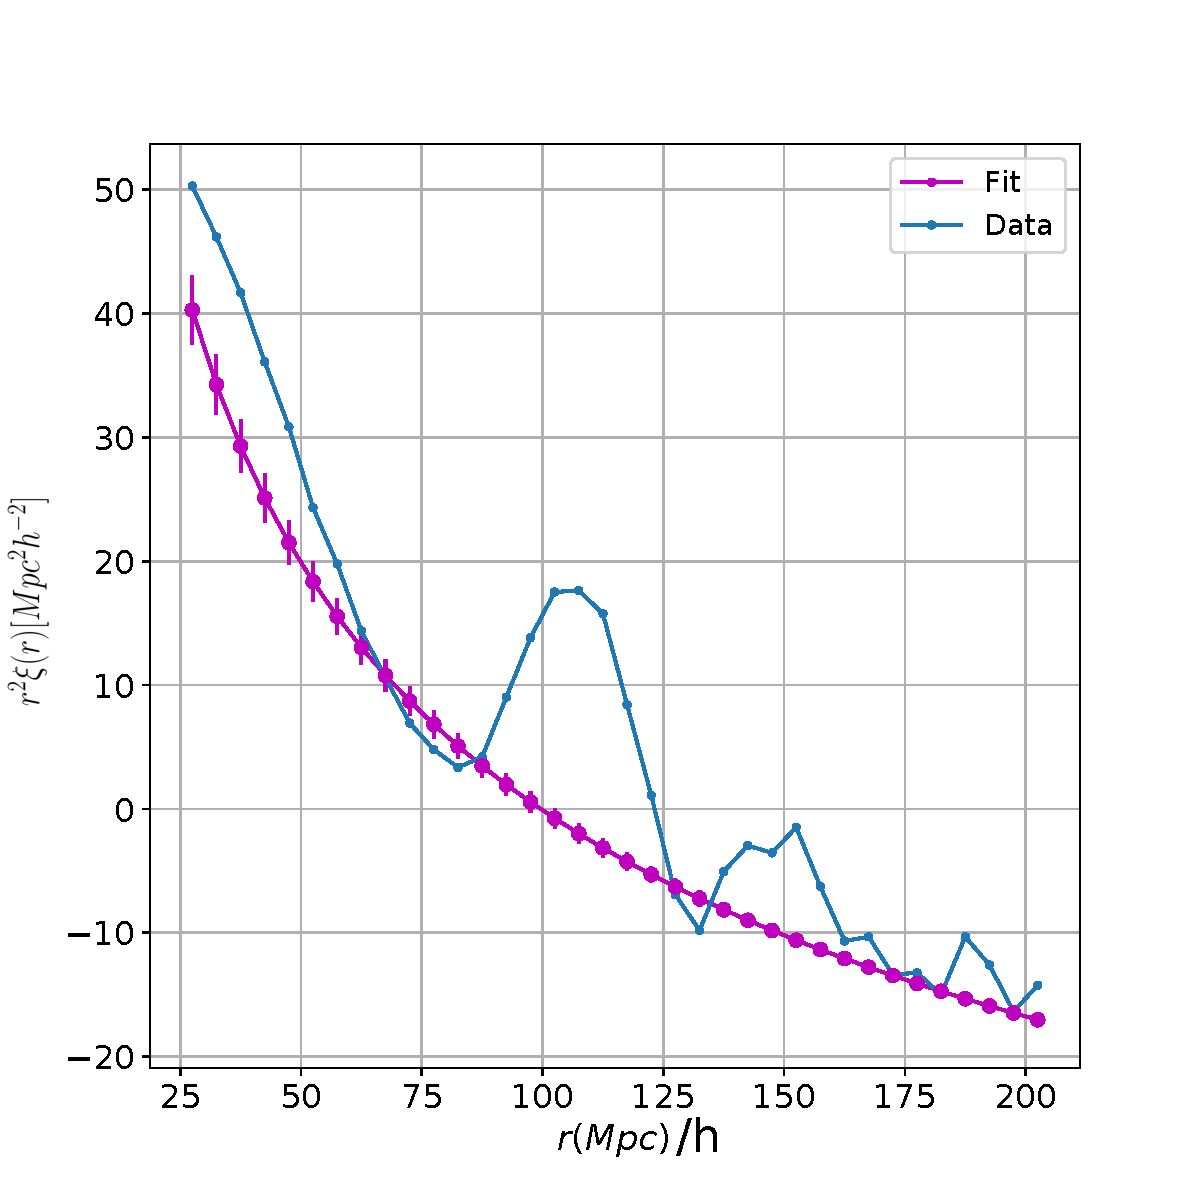
\includegraphics[width=85mm]{Images/chapter4/CF_fit_all_1e13.pdf}&
    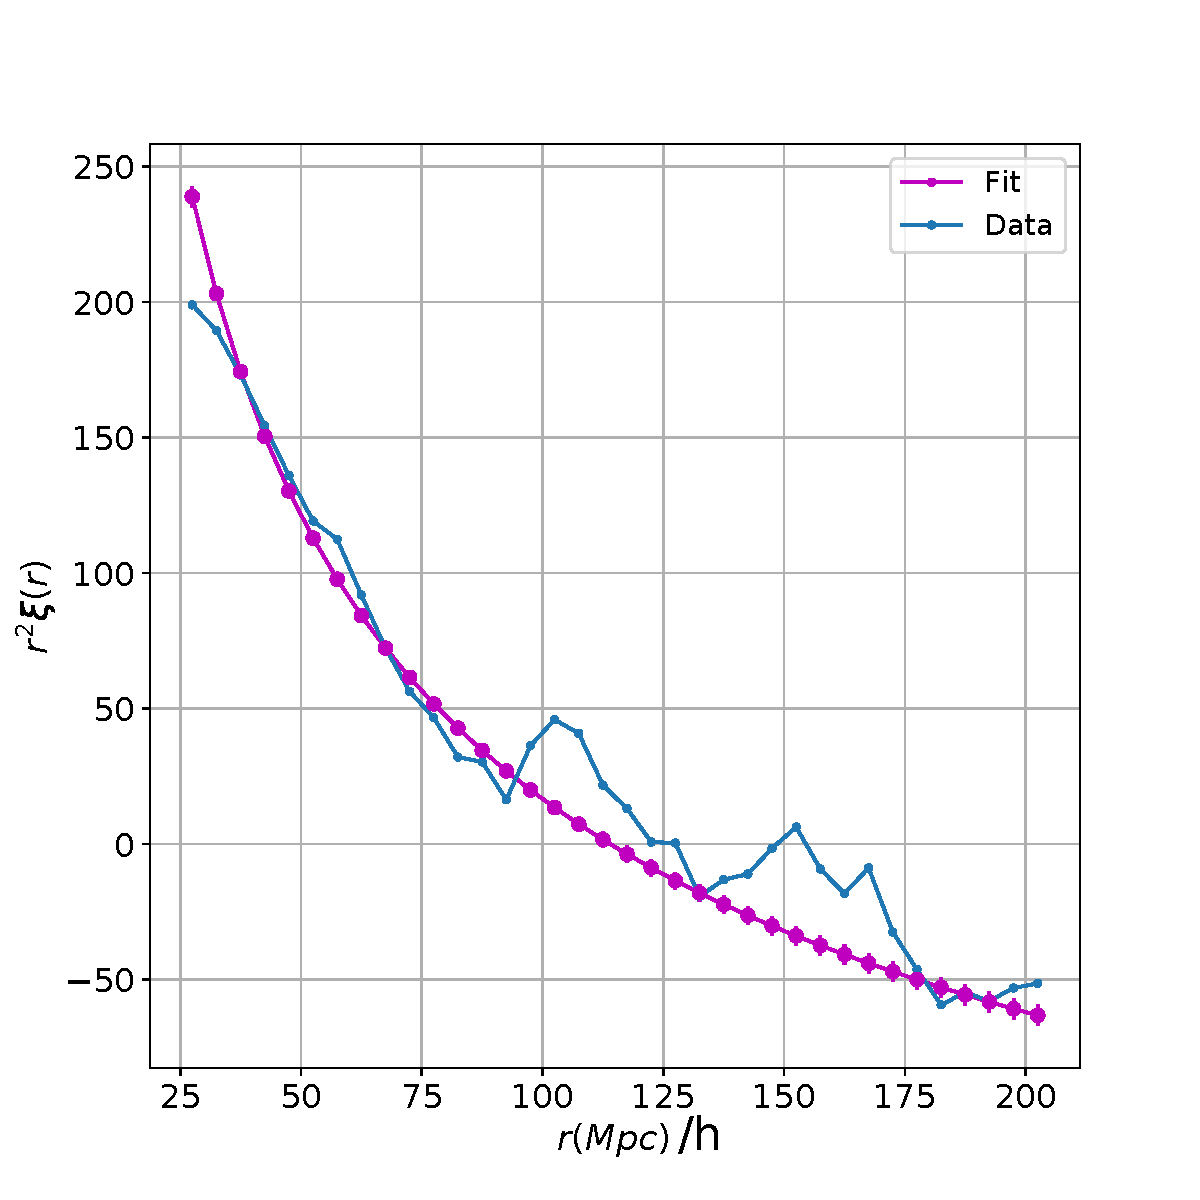
\includegraphics[width=85mm]{Images/chapter4/CF_fit_all_1e14.pdf}
    \end{array}$
  %\end{center}
   \caption{The correlation functions for populations thick $1$, $2$, $3$ and $4$ 
   are displayed from the upper left to the lower right. For each population 3 runs with 12 bins
   were carried out. }
   \label{CFall}
\end{figure}


where $\lambda$ and $a_0$ are the parameters found with the fit. 
The theoretical function used to adjust $\xi(r)$ was already shown in \ref{powlaw}. 
Since it is is a power law function, an easier way to carry out the fit is on 
logarithmic scale. In this way, it is performed a linear fit: $a r +b$. 
But, the values of the CF can be negative. Then, to avoid any trouble a $\Delta$ value 
is summed to the CF to get only positive values before perfoming the fit. 

When the coefficients $a$ and $b$ are obtained, we can recover the initial parameters
$\lambda$ and $a_0$  by considering the fact that $\gamma = a$ and $a_0=\exp(-b)$. 
Now, replacing the parameters in the expression \ref{CF_r2} and subtracting the amount $\Delta$, 
the CF can be plotted. 

This procedure is repeated to obtain the fit for every population and 
all of its realizations. In the figure \ref{CFall} some of the fits 
obtained for the samples are displayed. Here, 
one important thing is to get a measure of the robustness of the fit. Hence, 
error bars are calculated using the different realizations of the CF, i.e.,
the standard deviation is obtained. 
The error bars are shown for every figure of \ref{CFall} but 
because of the similarities of the fits they are almost no visible. 
So the CF fits are considered robust enough.  

In all of the CFs in \ref{CFall} there are visible two bumps, the first one
corresponds to the BAO since it agrees with the value observed of BAO
peak as it was shown in figure \ref{ps_cf}.
Also the position coincides with the BAO position measured for galaxy clusters, 
a mass range we are considering in our populations. 

Something to highlight is that in the population $q_2$ de $1e12$ 
there is no separation of this two bumps, making more difficult to recognize the BAO signal. 
It also happens with the population $2$ not shown in this figure. This 
was precisely the reason to study in more detail the effect of the mass bins in the CF estimation 
and thus the BAO bump. 


\subsection{BAO fit}

Since the measure of our interest is the BAO bump, it becomes necessary
to extract it from the CF and thus to be able to obtain the properties of 
BAO we are looking for to analyse. In this direction, a correlation function 
model can be useful  

\begin{equation}
CF(r) = \xi(r) - \Delta + GF(r,A,\mu,\sigma)
\end{equation}

the term $\xi(r)$ corresponds to the theoretical form shown in \ref{powlaw},
for us it is recovered from the CF fit divided by $r^2$. 
The second term is the one that it is summed to the CF as was explained
in the previous section, so it must be subtracted here. 
The function $GF$ is a gaussian fit that reproduces the BAO shape recovered 
from the correlation function. 

\[GF(r,A,\mu,\sigma) = Ae^{-(r-\mu)^2/(2\sigma^2)}\]

This model where BAO is fitted with a gaussian function is proposed in \cite{BAO_model}. 

Then, the next steps are followed to recover the BAO bump for every population. 
The median of the realizations is taken as the principal CF and the standard
deviation is obtained through the realizations.

\begin{itemize}

\item[1)] The term $\Delta$ is substracted from the CF fit. After the function
is divided by $r^2$ obtaining $\xi(r)$. 

\item[2)] The function $\xi(r)$ is substracted from the estimated CF leaving
the signal of the two bumps. 

\item[3)] Only the points corresponding to the first bump located around $105$ Mpc 
are selected. 

\item[4)] A gaussian fit of the first bump is performed. Only the more central points
of the signal are considered since the outer ones are the noiser parts of the signal. This noise 
could be diminished using more realizations per population. 

\item[5)] The fit is also performed for all the realizations, the same points
considered for the BAO signal fit of the mean CF are taken for the remaining realizations. 

\item[6)] The parameters amplitude $A$, mean $\mu$ and standard deviation $\sigma$ are
obtained for every population and the realizations. 

\end{itemize}

The parameters that characterizes the BAO bump are the amplitude $A$, the position
$\mu$ and the width $2\sigma$. In the figure \ref{BAO_fit} some fits of the BAO
signal are shown. It can be noticed that the points that correspond to the BAO
bump have a gaussian like distribution. The Gaussian fits performed are also shown
with the parameters found showing. It can be noticed a good accordance between 
the data and the fit obtained. 
The error bars displayed were obtained through the BAO fits performed for the
different realizations, with them the standard deviation per population was found.  


\begin{figure}[htbp]
   %\begin{center}
   $
    \begin{array}{ll}
    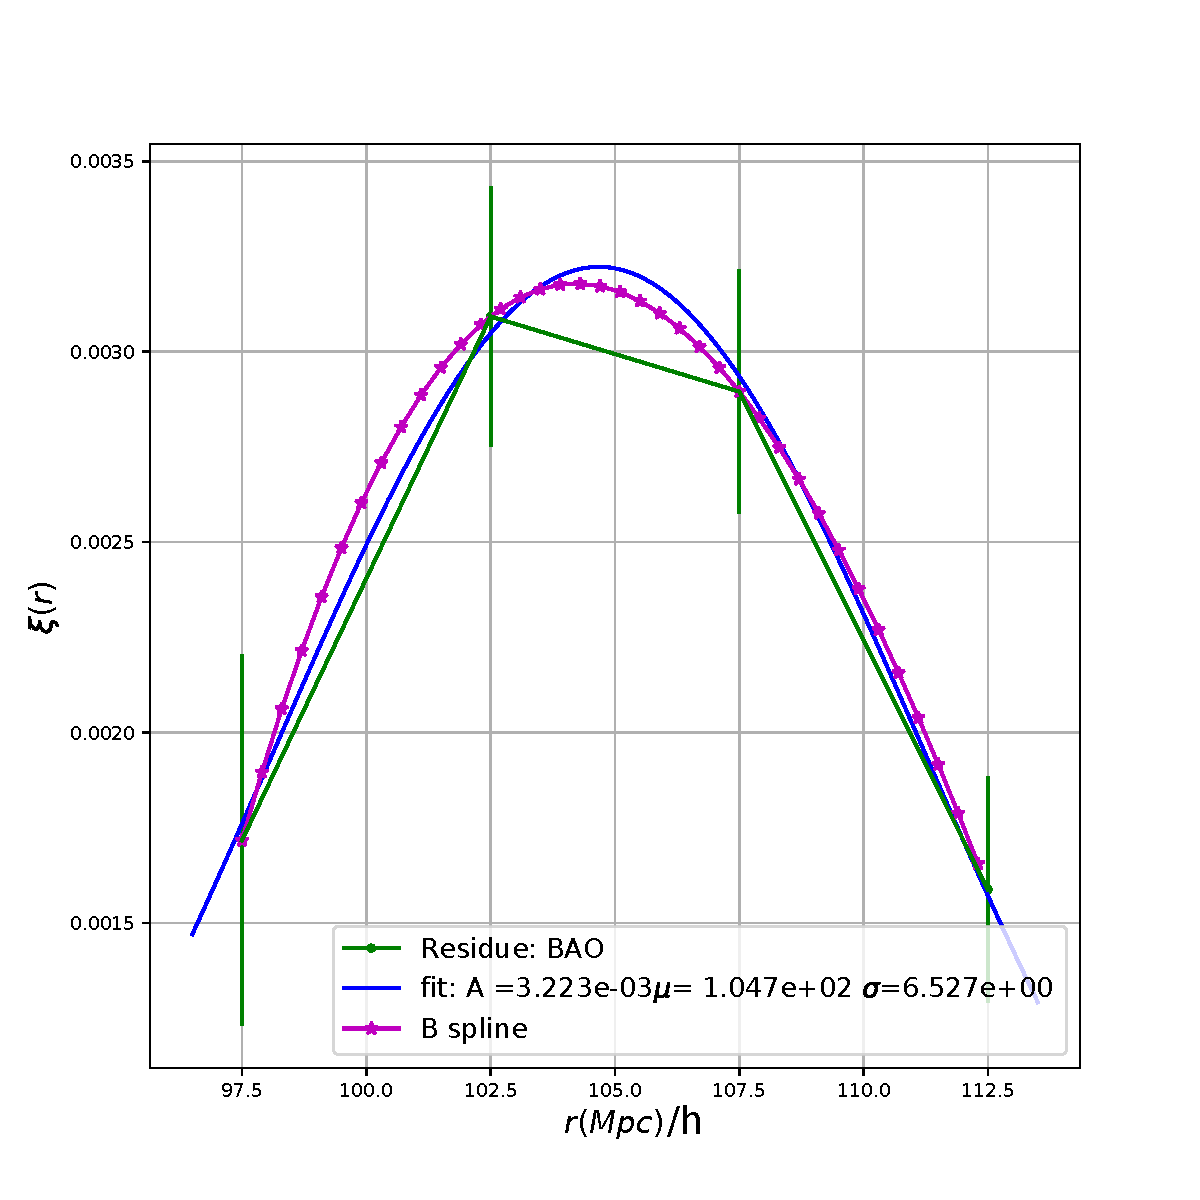
\includegraphics[width=85mm]{Images/chapter4/BAO_1e14.pdf}&
    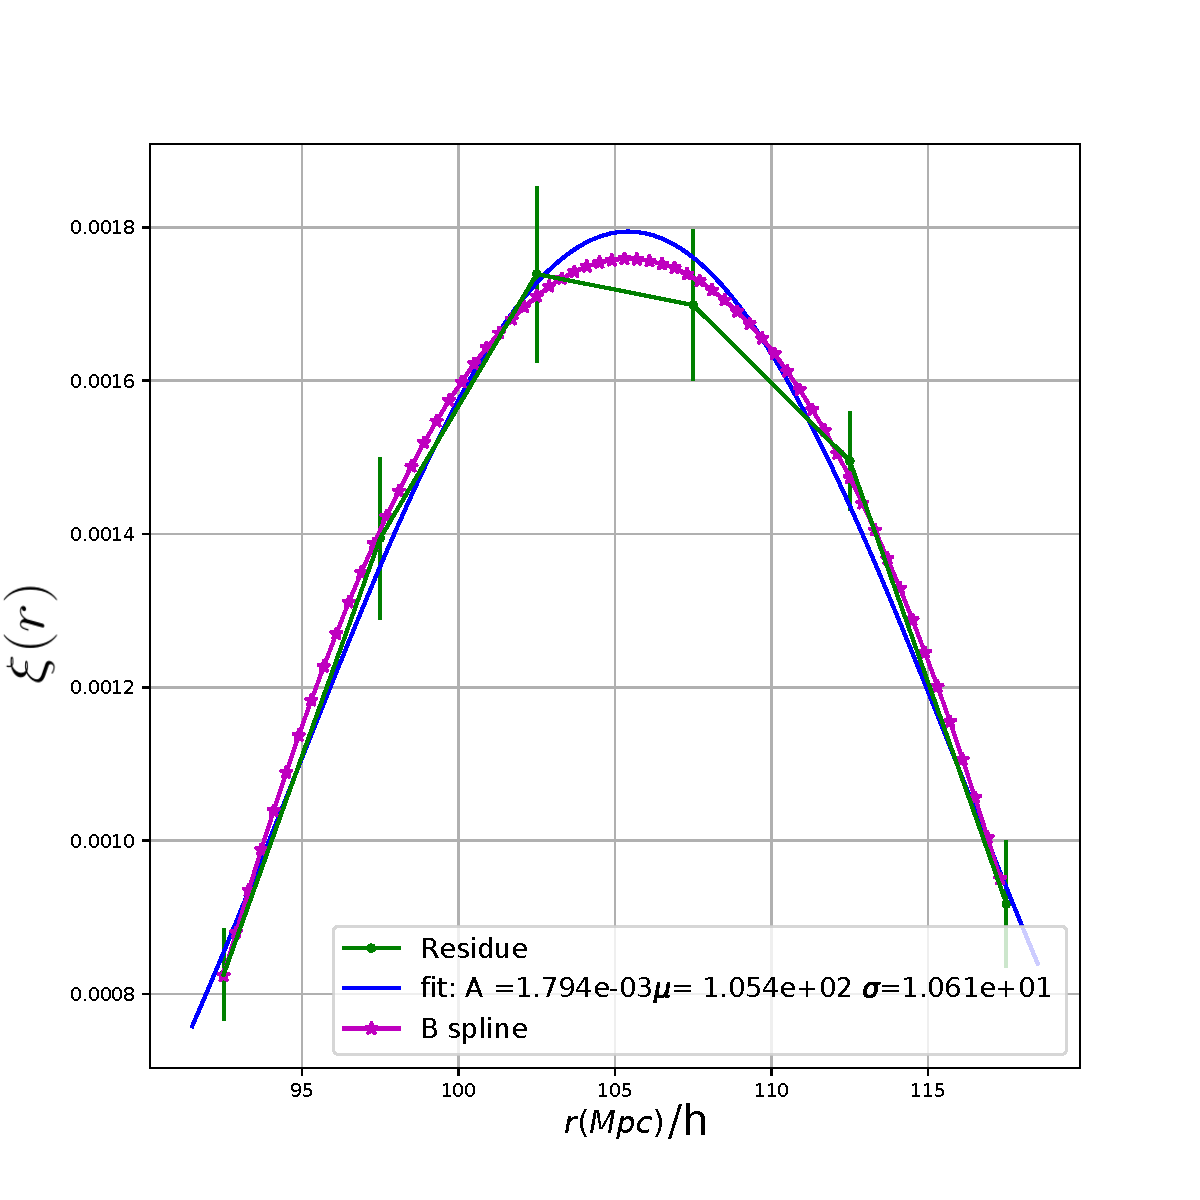
\includegraphics[width=85mm]{Images/chapter4/BAO_1e13.pdf}\\
    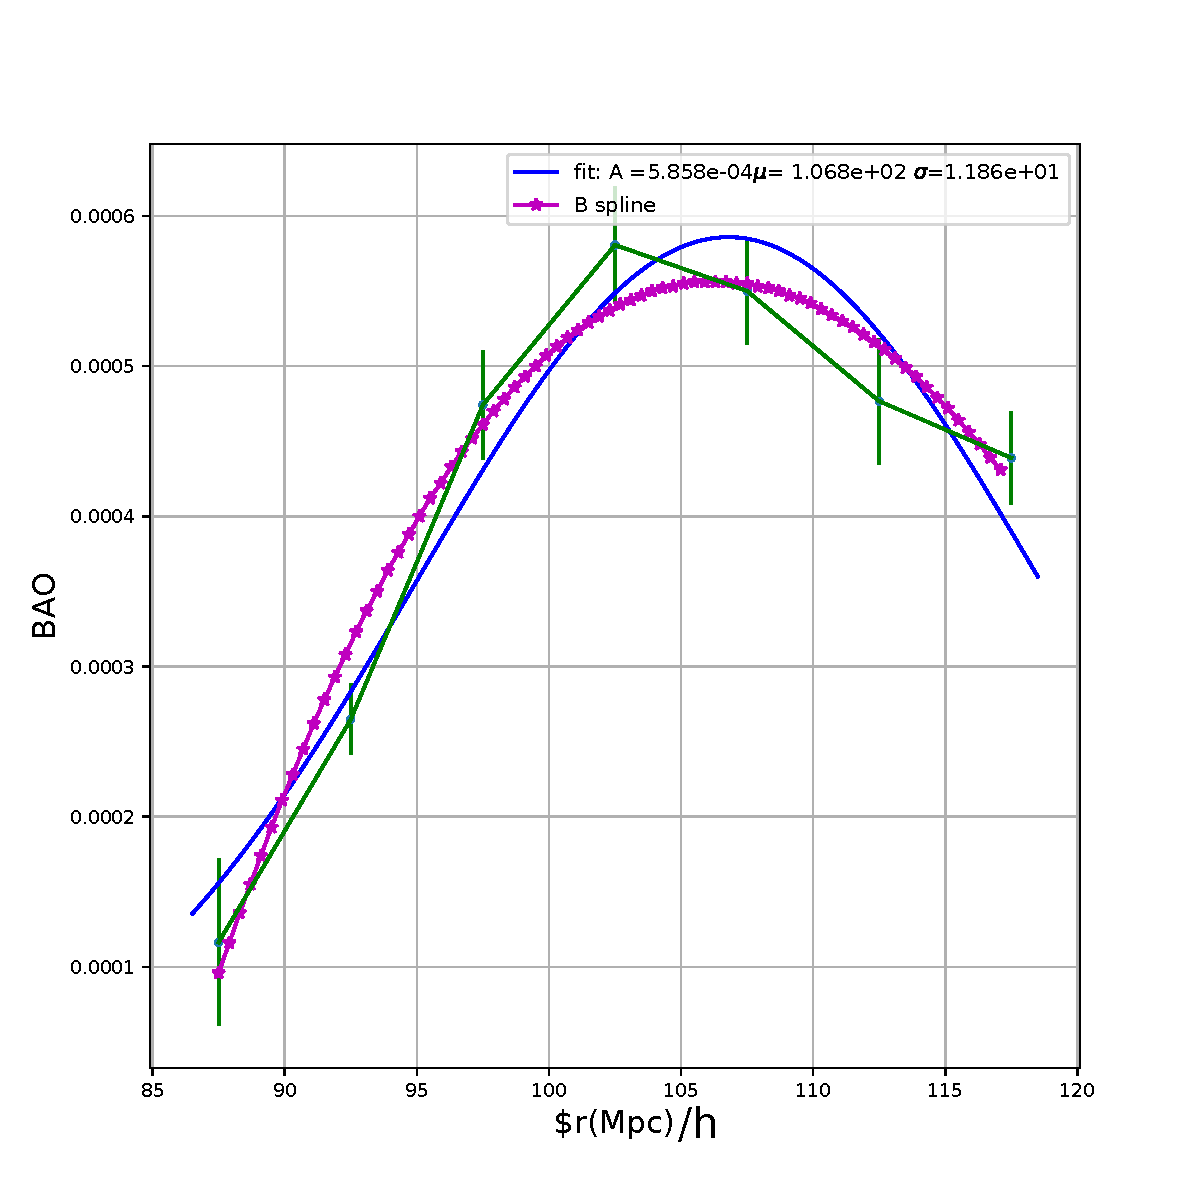
\includegraphics[width=85mm]{Images/chapter4/BAO_1e12_q4.pdf}&
    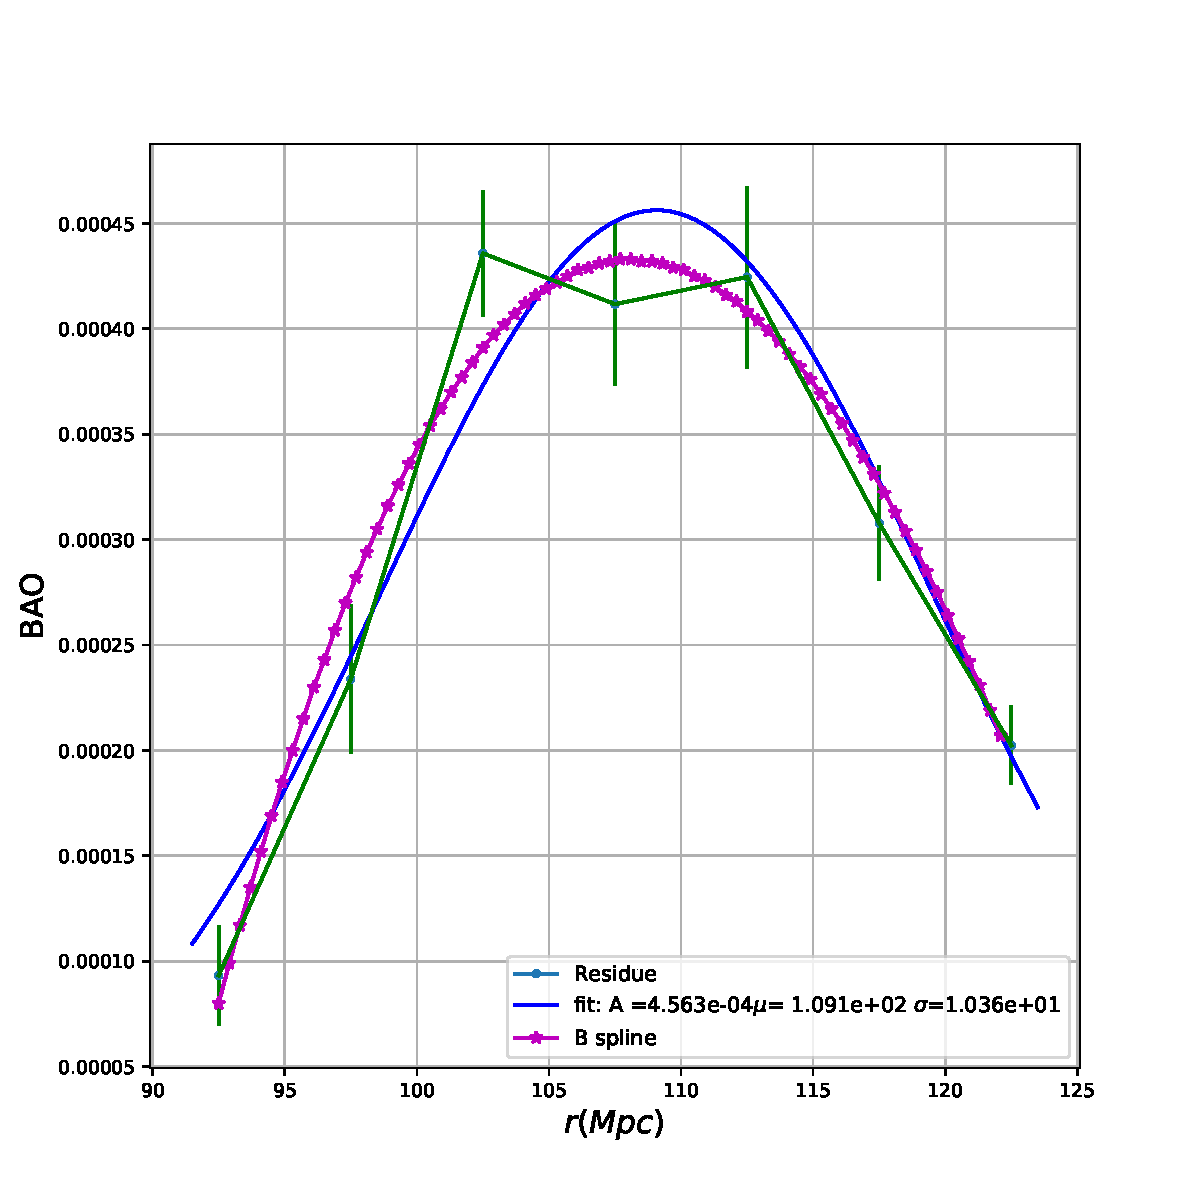
\includegraphics[width=85mm]{Images/chapter4/BAO_1e11_q1.pdf}
    \end{array}$
  %\end{center}
   \caption{ BAO signal for population 4, 3, $q_4$ of $1e12$ and $q_1$ of $1e11$ from
   upper left to lower right. }
   \label{BAO_fit}
\end{figure}

For every figures displayed in plot \ref{BAO_fit}, there is a curve labeled as B spline.
This fit was obtained using basis splines. It has a different behavior than the one observed 
for the Gaussian fit. At least in general terms, it fits better the BAO signal recovered.
Furthermore, there is a difference in the main peaks of the two fits 
performed, Gaussian and basis spline fit. Despite the difference between the peaks, the
functional form obtained for the properties is similar. This will be shown in the next section. 

\section{ BAO properties in the populations of MDPL }

As mentioned previously, the BAO peak is clearly detected for every population 
and the fit to the BAO signal was properly calculated using a Gaussian function. 
Let us see the situation in more detail. There are different populations, each of 
them have the ranges in mass shown in the beginning of this chapter.
  
For the thick bins, we are considering per population, more massive halos each 
time. That way, we are be able to analyze if there is an effect on the properties of 
BAO obtained for each population. 
It is important to take into account that more massive halos trace higher density 
peaks in the matter density field. This should lead, in principle, to a stronger 
correlation in the most massive populations compared with the less massive ones. 
Thus, a better detection of the BAO signal. In the left figure \ref{prop1} an increase of the amplitude of the BAO for more massive halos is obtained as precisely expected for a stronger 
correlation. 

\begin{figure}[h]
   %\begin{center}
   $
    \begin{array}{cc}
    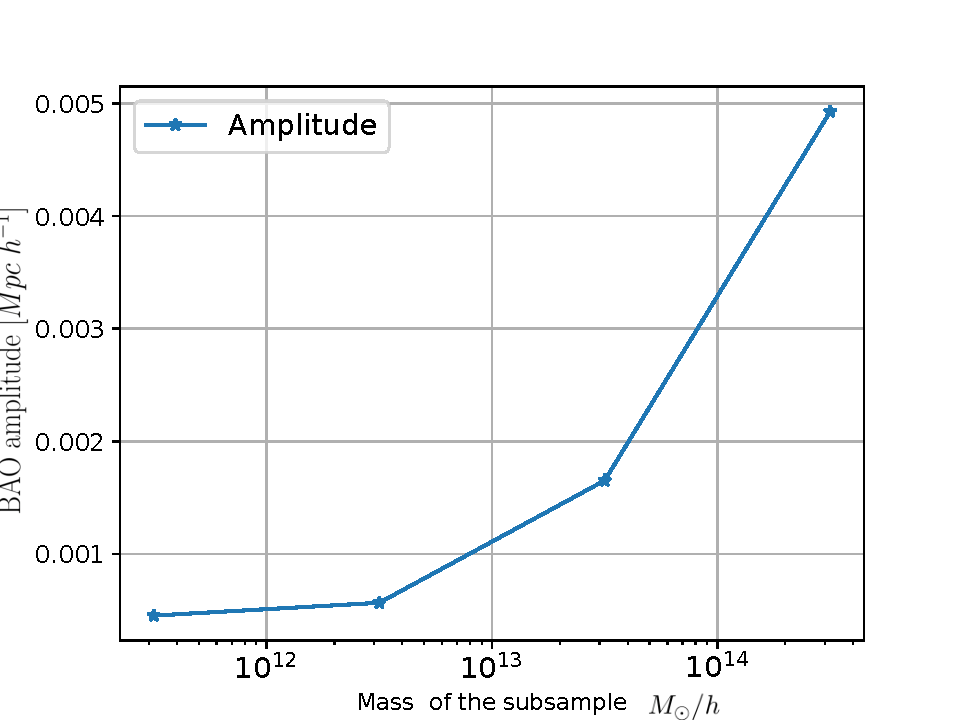
\includegraphics[width=78mm]{Images/chapter4/Amp_vs_Mh.pdf}&
    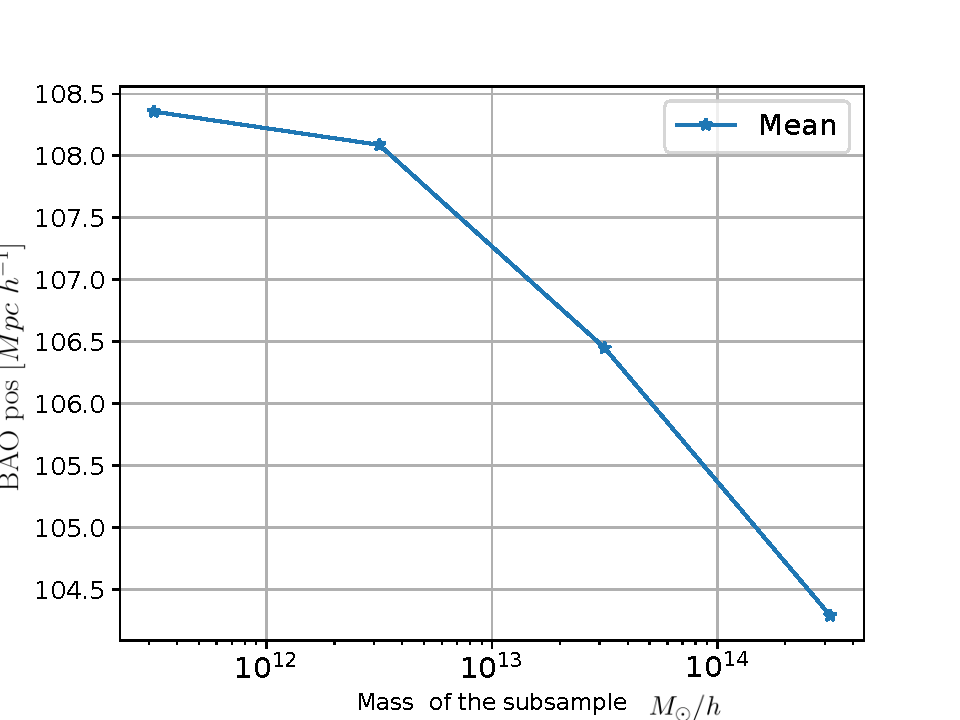
\includegraphics[width=78mm]{Images/chapter4/Pos_vs_Mh.pdf}
    \end{array}$
  %\end{center}
   \caption{\small In the left panel the amplitude of BAO in function of the mass of the thick populations 
   is shown. In the right one the position of BAO in function of the mass of the thick population is displayed.}
   \label{prop1}
\end{figure}

The initial position of the BAO depends on the sound horizon scale as mentioned in \ref{SH},
but as explained in the model exposed in \ref{shiftBAO}, this position changes due to
nonlinear effects. Now, the plot in the left of \ref{prop1} shows the position of the 
BAO in function of the halo mass. It can be noticed a decrease in the value of the position
as the halo mass increase. This behavior could be expected due to nonlinear gravitational 
collapse. The velocity field causes a movement of the BAO peak to smaller scales 
for the nonlinear regime. In this case, this corresponds to the 
smaller halo masses for which the density modes are coupled among them. 
The porcentual difference is around $3.8\%$. This is
precisely of the same order of magnitude found in \cite{motion}. This result contributes 
in a different way as \cite{motion} since they consider cosmological boxes with a very
small resolution $640^3$ in contrast with the populations used in this study. Furthermore,
we study the BAO behavior for a more extended mass range and this could let us see 
the effect of BAO properties in the nonlinear range. 

%**********************************************************************************************************************
\begin{figure}[htbp]
       \centering

    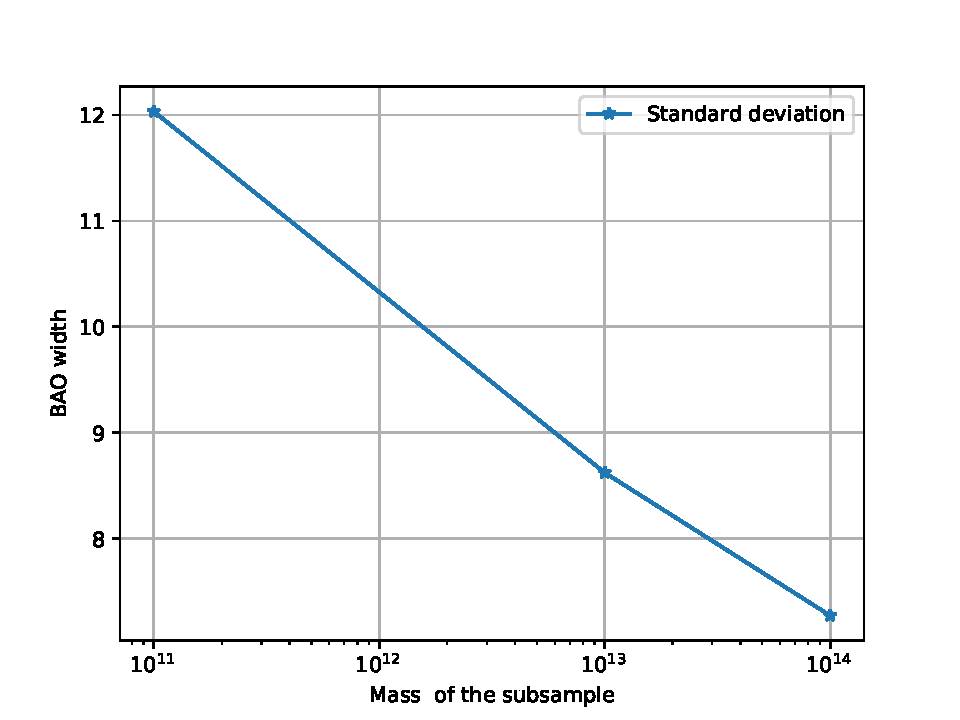
\includegraphics[width=90mm]{Images/chapter4/Width_vs_Mh.pdf}
\caption{\small Width of BAO versus the masss of the thick populations.}
       \label{sigm1}
 \end{figure}
%**********************************************************************************************************************

But not only the velocity field causes a shift of the BAO peak due to nonlinear evolution, 
there is a change of the width of the BAO peak. In order to understand this, let us consider
that the density field is affected by the dispersion of velocities and thus the correlation 
function obtanied. In this scenario, when we are considering halo populations with smaller 
masses, it is expected a bigger dispersion of the velocities compared with the populations 
with bigger masses. 	This occurs due to more massive halos are harder to move, thus the 
deviation from the mean velocity is not so big. At least,  compared  with the smaller halos 
that can have a wider range of velocities. 
To support this idea, let us consider the figure \ref{toy_pro} where a toy density profile 
is shown and separated in two parts, the one halo term  and the BAO signal. The one halo
term is affected by the dispersion of the velocities causing a broadening of this. Hence, 
a similar behavior is expected for the BAO signal. Thus, the BAO signal suffers a 
broadening but it depends on the halo mass considered. 


%**********************************************************************************************************************
\begin{figure}[htbp]
       \centering
    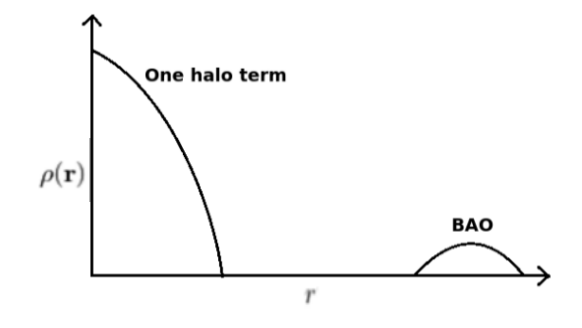
\includegraphics[width=70mm]{Images/chapter4/toy_pro.png}
\caption{\small Profile that includes one halo term and the BAO signal.}
       \label{toy_pro}
 \end{figure}
%**********************************************************************************************************************


\begin{comment}
Another important factor is the gravitational interaction among more massive halos.
Since larger masses exert greater gravitational attraction than smaller masses, 
the more massive halos should be closer among them, causing a smaller broadening
in the BAO peak compared with the less massive ones. This can be seen in the
figure \ref{sigm1} where the width of the BAO decreases with more massive halos.
But, the behavior of the population $2$ does not follow this tendency. Because of this,
the quarter and thin populations were created to study in more detail the effect of
the mass bins in the properties measure of BAO. 
\end{comment}


\begin{figure}[h]
   %\begin{center}
   $
    \begin{array}{cc}
    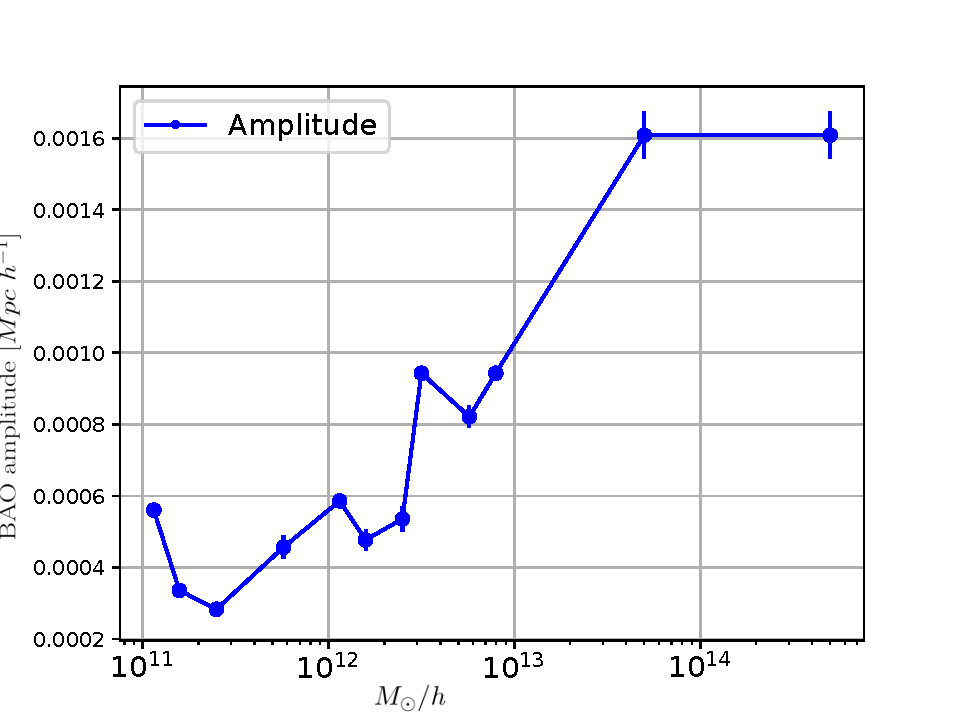
\includegraphics[width=78mm]{Images/chapter4/AmplitudevsMh2.pdf}&
    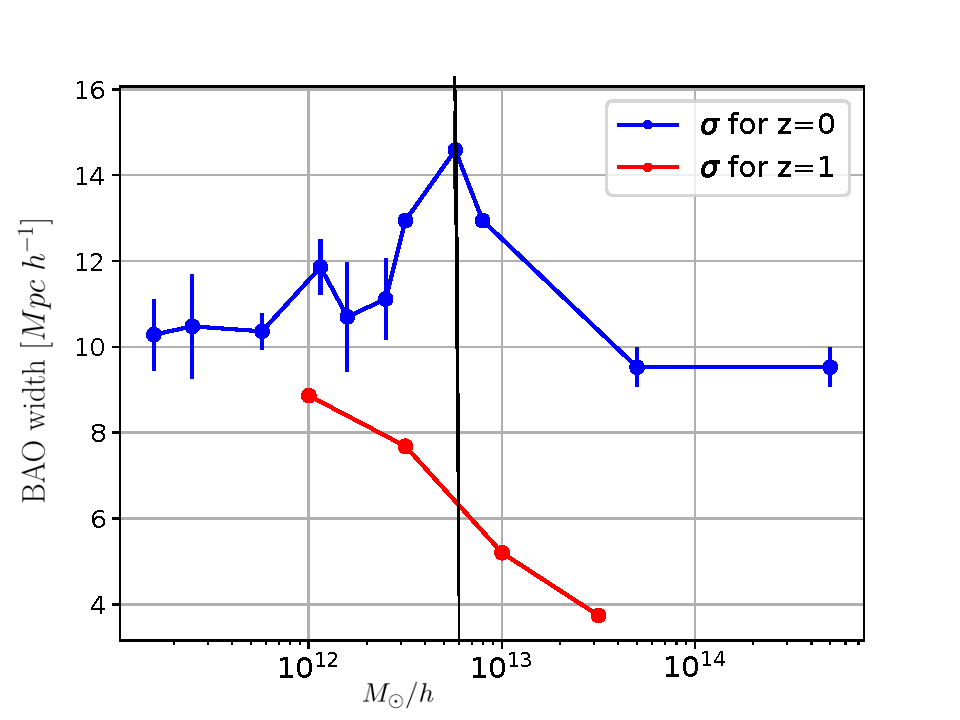
\includegraphics[width=78mm]{Images/chapter4/WidthvsMh2.pdf}
    \end{array}$
  %\end{center}
   \caption{\small In the left panel the amplitude of BAO in function of the mass of all populations 
   is shown. In the right one width of BAO versus the masss of the thick populations. }
   \label{prop2}
\end{figure}

%**********************************************************************************************************************
\begin{figure}[htbp]
       \centering

    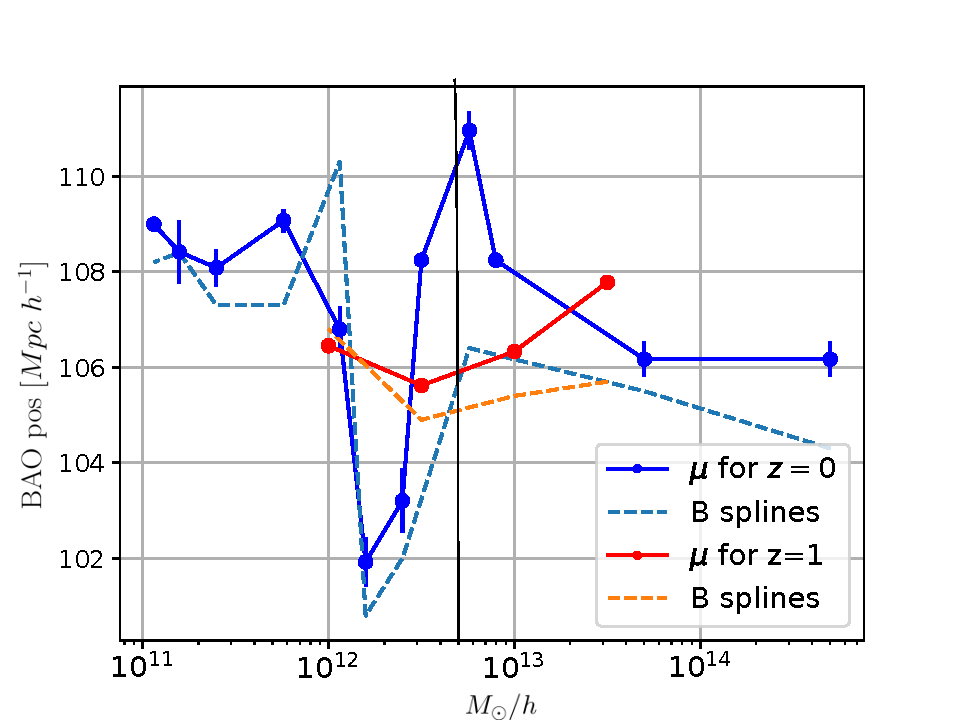
\includegraphics[width=100mm]{Images/chapter4/PosvsMh2.pdf}
\caption{\small The position of BAO in function of the mass of the thick population is displayed.}
       \label{sigm2}
 \end{figure}
%**********************************************************************************************************************


The BAO properties obtained for all the populations, except $1e11$ and $1e12$,
are plotted in the figures \ref{prop2} and \ref{sigm2}. It is noticed that when it is used
thiner masses bins, we do not recover the same tendency observed in the previous
figures. Let us start with the left figure of \ref{prop2}. In this case, there is
still a tendency of the amplitude to increase with an increase of the halo mass.
Though, for masses smaller than $\sim 10^{12.4}$, there is a more irregular behavior
compared with the one obtained for the thicker bins. 

Now, in the right figure of \ref{prop2}, it is not recovered the same behavior as \ref{sigm1}.
But, for halo masses bigger than $\sim 10^{12.4}$, the width of the BAO decreases
with mass. This was expected as explained for \ref{sigm1}. For masses smaller than
$\sim 10^{12.4}$, the nonlinear effects causes that there is no tendency of the 
data. 

In the figure \ref{sigm2}, shows the position of the BAO vs the halo mass.
In the case of the solid blue line, the populations considered are those ones that
belong to $z=0$, with the properties recovered using the Gaussian fit. To analyse it, 
let us again divide the figure in two regions. For halo masses bigger than $\sim 10^{12.4}$,
a similar behavior compared with \ref{prop1}, i.e., a decrease in the BAO position with
the increase of the halo mass. As was previously mentioned, this behavior is expected 
as explained in \ref{shiftBAO}. But, for masses smaller than $\sim 10^{12.4}$, it is not 
observed any specific tendency. It is in this region where the coupling among density
modes makes the nonlinear effects too big to extract any possible tendency. Hence, it 
is out of the purpose of this work to go deeper into the subject. 
A second curve is the discontinues blue line, it corresponds the same populations 
as the solid blue line. But, in this case, the position of the BAO was recovered
using a basis spline fit. This was perfomed to make the results obtanied
with the Gaussian BAO fit more robust. Although, there is a difference in the properties
recovered, this values are similar and also they behave in a similar manner. Thus,
the region for masses bigger than $\sim 10^{12.4}$ shows a decreases of the BAO position.
Hence, this supports the result obtained with the Gaussian fit. 
The red solid curve shows the BAO properties recovered for the populations with $z=1$.
It can be seen that BAO position does not change significantly due to the nonlinear 
effects are less prominent in this epoch. Similarly, the discontinues red line displays
the properties found for the same populations as the solid red line, but it recovers
the position using a basis spline fit. For both curves, there is not a notorious change 
in the position of the BAO. Hence, these two curves support the idea that nonlinear 
effects are causing a shift in the BAO position, not observed for $z=1$. 


Concluding, the properties recovered for the BAO using the thicker bins are behaving
as expected but they are possibly "masking" information of smaller mass scales. For this, 
the thiner bins provided us with a more accurate properties. This lead us to see that
for masses bigger than $\sim 10^{12.4}$, we recovered the expected tendency. But for
the smaller masses, the nonlinear effects do not let us extract any specific behavior
of the properties. A nonlinear behavior is dominating the BAO properties at these mass
scales. 

\section{Summary and conclusions}






















